\documentclass[10pt,letterpaper]{article}
\usepackage[margin=1in]{geometry}
\usepackage{amsmath,amssymb}
\usepackage{booktabs,tabularx,array,multirow}
\usepackage{graphicx}
\usepackage{xcolor}
\usepackage{tikz}
\usetikzlibrary{arrows.meta,positioning,calc}
\usepackage{pgfplots}
\pgfplotsset{compat=1.18}
\usepackage{enumitem}
\usepackage{fancyhdr}
\usepackage{caption}
\usepackage{microtype}
\usepackage[section]{placeins}
\usepackage[hidelinks]{hyperref}
\usepackage{orcidlink}
\renewcommand{\topfraction}{0.9}
\renewcommand{\bottomfraction}{0.8}
\renewcommand{\textfraction}{0.07}
\renewcommand{\floatpagefraction}{0.75}
\setcounter{totalnumber}{5}
\setcounter{topnumber}{3}

\captionsetup{font=small,labelfont=bf,labelsep=period}
\setlist{itemsep=2pt,topsep=3pt}
\renewcommand{\arraystretch}{1.15}
\newcolumntype{L}{>{\raggedright\arraybackslash}X}
\newcommand{\nd}{\textit{not documented}}
\newcommand{\pass}{pass}
\newcommand{\fail}{\textbf{fail}}

\definecolor{hdr}{gray}{0.45}
\pagestyle{fancy}
\fancyhf{}
\fancyhead[L]{\footnotesize\itshape\color{hdr}Evidence-Weighted Confidence}
\fancyhead[R]{\footnotesize\itshape\color{hdr}Zeinoun $\cdot$ Preprint, October 2026}
\renewcommand{\headrule}{{\color{hdr}\hrule width\headwidth height\headrulewidth}}
\fancyfoot[C]{\small\thepage}
\renewcommand{\headrulewidth}{0.4pt}


\begin{document}

\thispagestyle{empty}
\begin{center}
{\color{gray}\textsc{Preprint $\cdot$ Method and pre-registered experiments}}\\[14pt]
{\LARGE\bfseries Evidence-Weighted Confidence}\\[4pt]
{\large Auditable, Calibrated Scoring of LLM Outputs}\\[14pt]
{\large Issam Zeinoun~\orcidlink{0009-0007-4874-880X}}\\
{Independent Researcher}\\
{October 2026 $\cdot$ Version 3}
\end{center}
\vspace{6pt}

\begin{abstract}
\noindent Organizations that automate decisions with large language models (LLMs) face a basic problem: the confidence a model reports is not a probability. In our tests, when five current models said they were 93--99\% sure that a medical record supported a diagnosis code, they were right only 54--72\% of the time. Evidence-weighted confidence (EWC) fixes this by taking the judgment away from the model. The LLM only reads: it answers a short list of questions derived from the governing rules and quotes the text behind each answer. Code verifies the quotes, and a small logistic regression fitted on about 100 labeled cases turns the answers into a probability that comes with an audit trail.

In three pre-registered studies of ICD-10-CM coding on synthetic charts, ending with 200 held-out cases and five models, EWC's scores of 90\% or more were right 93--100\% of the time on every model, and EWC ranked cases far better than the models' own confidence (AUROC 0.90--1.00 against 0.59--0.77). It also let an inexpensive model match the best frontier result at about one fifteenth of the cost. The charts are synthetic; validation on real records is the next step.

\medskip\noindent\textbf{Keywords:} LLM evaluation; calibration; auditability; logistic regression; medical coding; risk adjustment.
\end{abstract}

% ---------------------------------------------------------------------------
\section{Introduction}

A confidence score is a claim about frequency: of all outputs scored 0.9, about 90\% should be correct. A number an LLM writes in its answer makes no such claim, and empirical work shows that verbalized confidence clusters in the 80--100\% range and is poorly calibrated~\cite{xiong}, more so after RLHF~\cite{leng}. In regulated work the problem is practical: a payer that auto-accepts a diagnosis code at ``95\% confidence'' must know that the 95\% means something and must be able to show an auditor why. Medical coding makes the stakes concrete: even strong models reproduce exact ICD-10-CM codes less than half the time~\cite{soroush}, so the question is which individual outputs to trust.

The method separates reading from judging. The LLM only reads: it answers rule-derived questions and quotes the text behind each answer. Code checks the quotes and turns the answers into features, and a small statistical model, fitted on labeled examples, turns the features into a probability that can be tested against outcomes.

\paragraph{Contributions.}
\begin{enumerate}
  \item \textbf{A design pattern} (Section~\ref{sec:method}): rule-derived questions answered by an LLM with verified quotes, encoded as 0/1 features and scored by a fitted logistic regression.
  \item \textbf{Confidence that means what it says} (Section~\ref{sec:calib}): on held-out charts and five models, the score's stated probability matched the observed rate of supported charts; the models' own confidence did not.
  \item \textbf{Fix the questions, not the model} (Section~\ref{sec:tuning}): a blind spot found on new charts was fixed by adding two rule-derived questions, with no change to any model.
  \item \textbf{Inexpensive models become usable} (Section~\ref{sec:cost}): with EWC, Claude Haiku 5.5 matched the best frontier result at a fraction of the cost.
\end{enumerate}

\paragraph{Related work.} Verbalized and token-probability confidence~\cite{xiong,leng} can be recalibrated after the fact~\cite{platt}, but stays a single opaque number; we use recalibrated stated confidence as a baseline. Checklist LLM judges such as CheckEval~\cite{checkeval} break an evaluation into yes/no questions and count the answers; EWC adds a third answer for \nd, verifies a quote for every answer and fits a weight to each. Concept bottleneck models~\cite{cbm} predict human-readable concepts and then the label; EWC has the same structure, with a pre-trained LLM as the concept extractor, so only outcome labels are needed. Weight-of-evidence scorecards and clinical point scores~\cite{good} add points per finding and fit them by logistic regression from structured data; EWC applies that scoring to evidence an LLM extracts from free text. Medical-coding benchmarks~\cite{soroush} measure overall accuracy rather than a probability per output, and this work complements criterion-level monitoring of AI in prior authorization~\cite{zeinoun}.

% ---------------------------------------------------------------------------
\section{Method}\label{sec:method}

\subsection{The rubric}

For each candidate output (here, a diagnosis code) a rubric defines evidence questions, each derived from a rule the decision is held to: for E11.22, the ICD-10-CM Official Guidelines for Coding and Reporting~\cite{guidelines}, the code's instructional note~\cite{tabular} and risk-adjustment documentation requirements. \textbf{Gate} questions must be answered yes for the code to be valid at all; \textbf{weighted} questions move the score once the gates pass. Every question has three answers: \textit{yes}, \textit{no} (the note says the opposite) and \nd{} (the note is silent), because a contradiction and silence are different evidence. Table~\ref{tab:rubric} lists the rubric used in the main study; Appendix~\ref{app:rubric} gives the full guidance the model receives.

\begin{table}[!htbp]
\centering\small
\caption{The E11.22 rubric (version 3). Gates must all be ``yes''; weighted questions become features of the fitted model.}\label{tab:rubric}
\begin{tabularx}{\textwidth}{@{}p{0.7cm}Lp{1.5cm}>{\raggedright\arraybackslash}p{4.6cm}@{}}
\toprule
ID & Question & Role & Rule it implements \\
\midrule
G1 & Is type 2 diabetes documented as a current diagnosis? & Gate & E10/E11 by type; untyped defaults to E11 (I.C.4.a) \\
G2 & Is CKD documented by the provider as an established diagnosis? & Gate & No uncertain or resolved diagnoses (IV.H, IV.J) \\
R1 & Was the patient seen face to face by an MD, DO, NP or PA? & Gate & Risk-adjustment acceptable encounter and provider \\
R2 & Is the note signed with a professional credential? & Gate & Risk-adjustment signature requirement \\
Q1 & Is the CKD stage documented? & Weighted & ``Use additional code to identify stage'' (E11.22 note) \\
Q2 & Do the labs show eGFR below 60 on two results at least 90 days apart? & Weighted & Clinical validation used by auditors \\
Q3 & Does the provider attribute the CKD to diabetes? & Weighted & ``With'' presumes the link unless another cause is documented (I.A.15) \\
Q4 & Was the CKD addressed at this encounter (monitored, evaluated, assessed or treated)? & Weighted & Code conditions that affect care (IV.I, IV.J); MEAT audit convention \\
\bottomrule
\end{tabularx}
\end{table}

\subsection{From chart to probability}

Figure~\ref{fig:pipeline} shows the whole method on one chart. Only step 1 uses an LLM; every later step is deterministic and logged. Quote verification is a plain string match after normalizing case, spacing and punctuation.

\begin{figure}[!htbp]
\centering
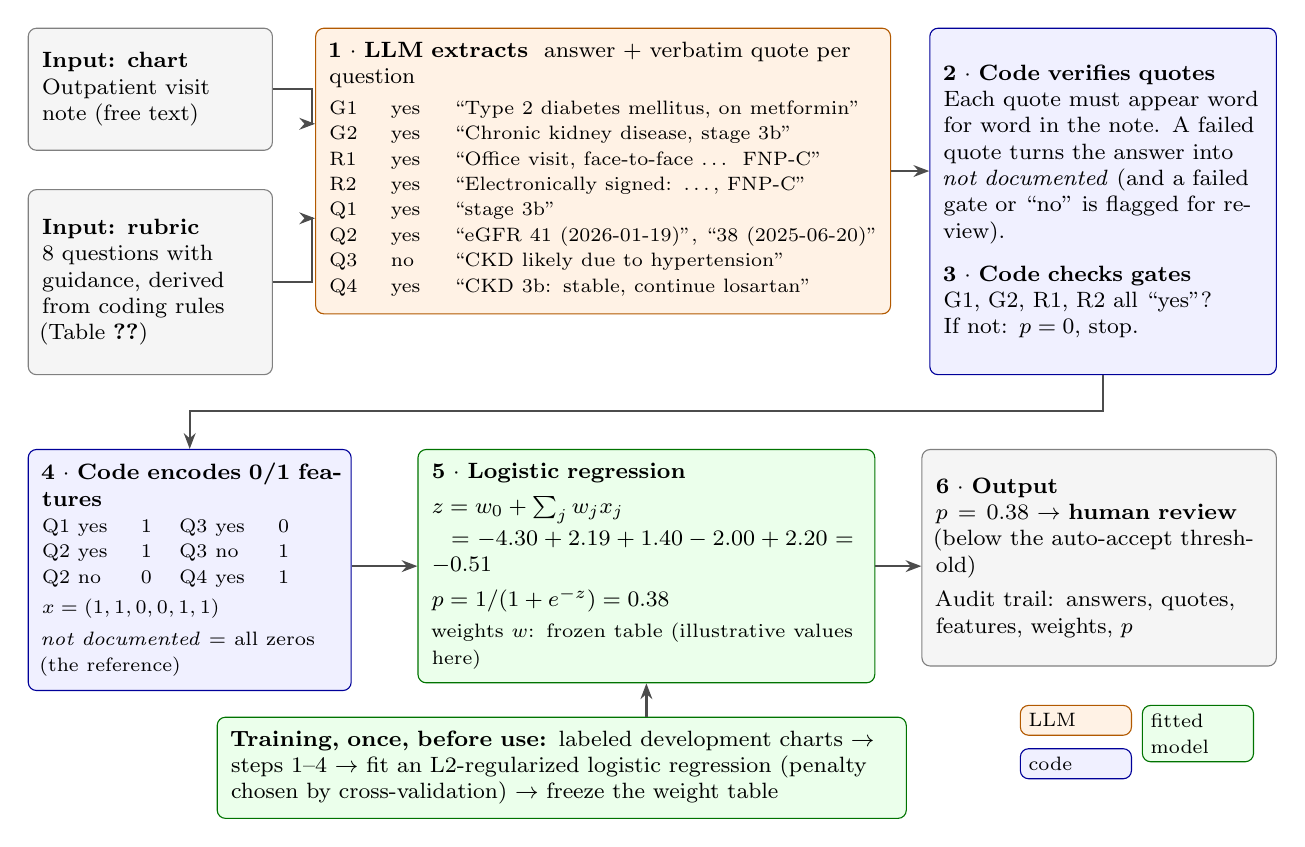
\begin{tikzpicture}[font=\footnotesize,
  box/.style={draw,rounded corners=3pt,align=left,inner sep=5pt,anchor=north west},
  llm/.style={box,fill=orange!10,draw=orange!70!black},
  code/.style={box,fill=blue!6,draw=blue!60!black},
  model/.style={box,fill=green!8,draw=green!45!black},
  plain/.style={box,fill=black!4,draw=black!50},
  arr/.style={-{Stealth[length=2mm]},thick,draw=black!70}]
% Row 1
\node[plain,text width=2.75cm,minimum height=1.55cm] (chart) at (0,0) {\textbf{Input: chart}\\Outpatient visit note (free text)};
\node[plain,text width=2.75cm,minimum height=2.35cm] (rubric) at (0,-2.05) {\textbf{Input: rubric}\\8 questions with guidance, derived from coding rules (Table~\ref{tab:rubric})};
\node[llm,text width=6.95cm] (extract) at (3.65,0) {\textbf{1 $\cdot$ LLM extracts} \ answer + verbatim quote per question\\[2pt]
\scriptsize
\begin{tabular}{@{}lll@{}}
G1 & yes & ``Type 2 diabetes mellitus, on metformin''\\
G2 & yes & ``Chronic kidney disease, stage 3b''\\
R1 & yes & ``Office visit, face-to-face \ldots{} FNP-C''\\
R2 & yes & ``Electronically signed: \ldots{}, FNP-C''\\
Q1 & yes & ``stage 3b''\\
Q2 & yes & ``eGFR 41 (2026-01-19)'', ``38 (2025-06-20)''\\
Q3 & no & ``CKD likely due to hypertension''\\
Q4 & yes & ``CKD 3b: stable, continue losartan''\\
\end{tabular}};
\node[code,text width=4.05cm,minimum height=4.4cm] (verify) at (11.45,0) {\textbf{2 $\cdot$ Code verifies quotes}\\Each quote must appear word for word in the note. A failed quote turns the answer into \nd{} (and a failed gate or ``no'' is flagged for review).\\[6pt]
\textbf{3 $\cdot$ Code checks gates}\\G1, G2, R1, R2 all ``yes''?\\If not: $p=0$, stop.};
% Row 2
\node[code,text width=3.75cm,minimum height=2.75cm] (encode) at (0,-5.35) {\textbf{4 $\cdot$ Code encodes 0/1 features}\\[2pt]
\scriptsize
\begin{tabular}{@{}lc@{\hspace{10pt}}lc@{}}
Q1 yes & 1 & Q3 yes & 0\\
Q2 yes & 1 & Q3 no & 1\\
Q2 no & 0 & Q4 yes & 1\\
\end{tabular}\\[2pt]
$x=(1,1,0,0,1,1)$\\[2pt]
\scriptsize \nd{} = all zeros (the reference)};
\node[model,text width=5.45cm,minimum height=2.75cm] (lr) at (4.95,-5.35) {\textbf{5 $\cdot$ Logistic regression}\\[3pt]
$z = w_0 + \sum_j w_j x_j$\\[2pt]
$\phantom{z}= -4.30 + 2.19 + 1.40 - 2.00 + 2.20 = -0.51$\\[3pt]
$p = 1/(1+e^{-z}) = 0.38$\\[2pt]
\scriptsize weights $w$: frozen table (illustrative values here)};
\node[plain,text width=4.15cm,minimum height=2.75cm] (out) at (11.35,-5.35) {\textbf{6 $\cdot$ Output}\\$p=0.38$ $\rightarrow$ \textbf{human review} (below the auto-accept threshold)\\[3pt]
Audit trail: answers, quotes, features, weights, $p$};
% Row 3: training
\node[model,text width=8.4cm] (train) at (2.4,-8.75) {\textbf{Training, once, before use:} labeled development charts $\rightarrow$ steps 1--4 $\rightarrow$ fit an L2-regularized logistic regression (penalty chosen by cross-validation) $\rightarrow$ freeze the weight table};
% arrows
\draw[arr] (chart.east) -- ++(0.5,0) |- ($(extract.west)+(0,0.6)$);
\draw[arr] (rubric.east) -- ++(0.5,0) |- ($(extract.west)+(0,-0.6)$);
\draw[arr] (extract.east) -- (verify.west|-extract.east);
\draw[arr] (verify.south) -- ++(0,-0.45) -| (encode.north);
\draw[arr] (encode.east|-lr.west) -- (lr.west);
\draw[arr] (lr.east) -- (out.west|-lr.east);
\draw[arr] (train.north-|lr.south) -- (lr.south);
% legend
\node[llm,text width=1.2cm,inner sep=3pt] at (12.6,-8.6) {\scriptsize LLM};
\node[code,text width=1.2cm,inner sep=3pt] at (12.6,-9.15) {\scriptsize code};
\node[model,text width=1.2cm,inner sep=3pt] at (14.15,-8.6) {\scriptsize fitted model};
\end{tikzpicture}
\caption{Evidence-weighted confidence on one chart. The LLM answers the rubric's questions with quotes (1); code verifies the quotes (2), applies the gates (3) and turns the weighted answers into 0/1 features (4); a logistic regression with a frozen weight table turns the features into a probability (5), which routes the chart and is logged with its evidence (6). The weights are fitted once on labeled development charts. Here a documented other cause (Q3 = no) pulls a chart that is otherwise well documented down to 0.38.}\label{fig:pipeline}
\end{figure}

\paragraph{Encoding.} Each weighted question contributes one indicator per answer, $\mathbf{1}[\text{yes}]$ and $\mathbf{1}[\text{no}]$; \nd{} is the reference, so silence counts 0 and each weight is the change in log-odds relative to the note being silent. Q1 and Q4 have no ``no'' answer, so the model has six features.

\paragraph{Scoring and fitting.} The probability is $p=\sigma(w_0+\sum_j w_j x_j)$. The weights are fitted on development charts that pass the gates, by L2-regularized logistic regression with the penalty chosen by repeated stratified 5-fold cross-validation, then frozen before the test split is scored. Three properties make this form a good fit for evidence. Contributions add on the log-odds scale, so many findings never push the probability past 0 or 1. Absence counts: because silence is the reference, a large weight for ``yes'' means that its absence lowers the score. And because all weights are fitted together, two answers that restate the same fact share credit instead of being counted twice. The full fitting procedure, with a reference implementation, is in the extended version of this paper~\cite{ewc1} and the study repository.

\paragraph{Routing.} Charts above a threshold chosen on development data for 95\% precision are accepted automatically; the rest go to human review. A chart flagged by the verification rule is never auto-accepted.

\subsection{Three charts}

Table~\ref{tab:three} and Figure~\ref{fig:logistic} show why the score separates charts that a stated confidence would rate alike: each of these mentions both diabetes and CKD, and a model asked for its confidence would likely rate all three 85--95\%.

\begin{table}[!htbp]
\centering\small
\caption{Three charts that pass the gates, scored with illustrative weights ($w_0=-4.30$; Q1 yes $+2.19$; Q2 yes $+1.40$, no $-1.20$; Q3 yes $+0.90$, no $-2.00$; Q4 yes $+2.20$). n.d.\ = \nd.}\label{tab:three}
\begin{tabularx}{\textwidth}{@{}p{3.6cm}p{3.6cm}Lc@{}}
\toprule
Chart & Answers & Log-odds & $p$ \\
\midrule
Complete documentation & Q1 yes, Q2 yes, Q3 yes, Q4 yes & $-4.30+2.19+1.40+0.90+2.20=2.39$ & 0.92 \\
Problem-list mention only & Q1 yes, Q2 n.d., Q3 n.d., Q4 n.d. & $-4.30+2.19=-2.11$ & 0.11 \\
CKD attributed to hypertension & Q1 yes, Q2 yes, Q3 no, Q4 yes & $-4.30+2.19+1.40-2.00+2.20=-0.51$ & 0.38 \\
\bottomrule
\end{tabularx}
\end{table}

\begin{figure}[!htbp]
\centering
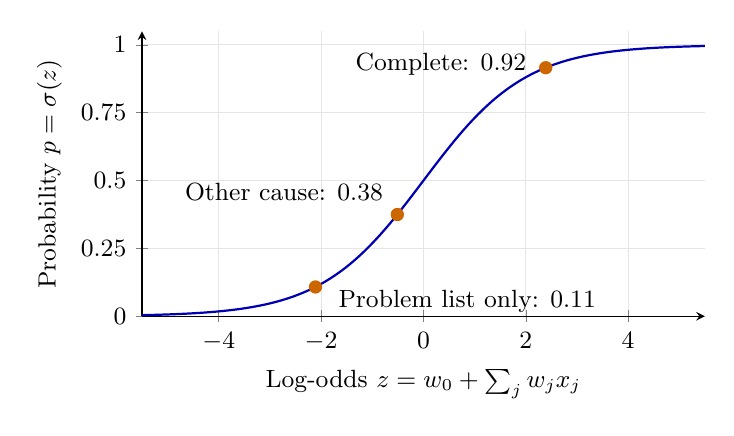
\begin{tikzpicture}
\begin{axis}[width=0.72\textwidth,height=5.2cm,xmin=-5.5,xmax=5.5,ymin=0,ymax=1.05,
  xlabel={Log-odds $z=w_0+\sum_j w_j x_j$},ylabel={Probability $p=\sigma(z)$},
  ytick={0,0.25,0.5,0.75,1},axis lines=left,grid=major,grid style={black!10},font=\small]
\addplot[domain=-5.5:5.5,samples=120,thick,blue!70!black]{1/(1+exp(-x))};
\addplot[only marks,mark=*,mark size=2.2pt,orange!80!black] coordinates {(2.39,0.916) (-2.11,0.108) (-0.51,0.375)};
\node[anchor=east,font=\small] at (axis cs:2.2,0.93) {Complete: 0.92};
\node[anchor=west,font=\small] at (axis cs:-1.85,0.055) {Problem list only: 0.11};
\node[anchor=south east,font=\small] at (axis cs:-0.6,0.39) {Other cause: 0.38};
\end{axis}
\end{tikzpicture}
\caption{The three charts of Table~\ref{tab:three} on the logistic curve. Each chart's evidence adds up to a log-odds score $z$, and the sigmoid turns it into a probability. The same change in evidence moves the probability most in the middle of the curve and least at the extremes.}\label{fig:logistic}
\end{figure}

% ---------------------------------------------------------------------------
\section{Experiments}\label{sec:experiments}

\subsection{Design}

An earlier version of this paper~\cite{ewc1} presented the method and the evaluation protocol before any experiment was run. Three studies followed, each pre-registered: hypotheses, pass marks and analysis rules were fixed in advance, prompts, rubric, weights, recalibration maps and thresholds were frozen with cryptographic hashes before any test call, and each model's test split was evaluated once. Deviations from the plan are listed in the Limitations. Code, data, pre-registrations, freeze records and a change log are at \url{https://github.com/izeinoun/rubric_for_medical_coding}.
\begin{enumerate}
  \item \textbf{Study 1, pilot:} 200 charts (140 development, 60 test), a six-question rubric, GPT-5.4 and Gemini 3.8 Flash.
  \item \textbf{Study 2, transfer test:} the frozen pilot pipeline on 300 harder charts; stopped after a first stage of 100 charts, as its pre-registration allowed, once it had shown what the rubric missed.
  \item \textbf{Study 3, main study:} 350 charts (150 development, 200 test), rubric version 3, five models. All results below are from study 3 unless stated.
\end{enumerate}

\paragraph{Data.} Synthetic outpatient notes (median about 3,400 characters, with format noise such as broken lines and copied-forward sections) in eight families: the pilot scenarios; copied-forward plans; harder gates (untyped, insulin-treated, type 1 or secondary diabetes, CKD resolved after transplant); lab and date edge cases; cause attribution; failures the pilot rubric could not see (nurse-only visits, unsigned notes, chart-review e-consults); borderline ``addressed'' wording; and 50 hard cases (conflicting statements, stage contradicted by labs, dialysis, unclear statements). The test split has 200 charts (117 supported), none seen by any model before.

\paragraph{Labels.} A chart is supported only if type 2 diabetes is documented; CKD is an established diagnosis; CKD is addressed at this visit; CKD is not attributed to another cause \emph{instead of} diabetes; the visit was face to face with an MD, DO, NP or PA; and the note is signed with a credential. ``Addressed'' follows the MEAT reading set by the study lead (a copied plan line with a status counts; ``see nephrology note'' alone does not), and an unresolved contradiction about CKD or the diabetes type makes a chart unsupported. The rules were set by the study lead with AI assistance.

\paragraph{Methods compared.}
\textbf{A}, the model's stated 0--100 confidence, raw and Platt-recalibrated on development data;
\textbf{C}, the same eight questions and guidance in the prompt, with the model told to base its confidence on them (one number, not recalibrated);
\textbf{B}, evidence-weighted confidence.
C is the fair comparison for B: both see exactly the same questions, so any difference comes from how the answers become a number.

\paragraph{Models.} GPT-5.4 (\texttt{gpt-5.4-2026-03-05}) and Gemini 3.8 Flash were pre-registered; Claude Sonnet 5.5, Claude Haiku 5.5 and Gemini 3.5 Flash-Lite were added afterwards, each under a written addendum filed before its first call, with its own development fit, freeze and single test evaluation. Each model made 11 calls per chart (five extraction runs, five stated-confidence runs, one criteria-guided run); the first run of each is scored.

\paragraph{Hypotheses and metrics (per model, test split; 95\% paired bootstrap intervals, 2,000 resamples).}
H1: B ranks better than recalibrated A by at least 0.10 AUROC, interval above 0.
H2: B ranks better than C, interval above 0.
H3: B's expected calibration error (ECE) is no higher than recalibrated A's and C's.
H4: B's development threshold gives at least 95\% precision on test.
The pre-registration predicted that H2 would likely fail for Gemini 3.8 Flash, where C had tied B on development data.

\subsection{Pre-registered results}

\begin{table}[!htbp]
\centering\small
\caption{Pre-registered checks, study 3 test split (200 charts per model). Precision of B at its frozen threshold, with charts auto-accepted and recall.}\label{tab:prereg}
\begin{tabularx}{\textwidth}{@{}lp{2.35cm}p{2.35cm}p{2.6cm}L@{}}
\toprule
Model & H1: B $-$ A AUROC & H2: B $-$ C AUROC & H3: ECE B / A / C & H4: B precision at threshold \\
\midrule
GPT-5.4 & 0.333 (0.243, 0.417) \pass & 0.443 (0.352, 0.530) \pass & 0.037 / 0.046 / 0.368 \pass & 0.935 (46 accepted, recall 0.37) \fail \\
Claude Sonnet 5.5 & 0.272 (0.193, 0.360) \pass & $-0.008$ ($-0.025$, 0.003) \fail & 0.021 / 0.067 / 0.090 \pass & 0.966 (119, recall 0.98) \pass \\
Claude Haiku 5.5 & 0.222 (0.147, 0.305) \pass & 0.077 (0.031, 0.131) \pass & 0.014 / 0.111 / 0.234 \pass & 0.967 (120, recall 0.99) \pass \\
Gemini 3.8 Flash & 0.353 (0.280, 0.434) \pass & 0.000 (0.000, 0.000) \fail & 0.002 / 0.108 / 0.036 \pass & 0.959 (122, recall 1.00) \pass \\
Gemini 3.5 Flash-Lite & 0.205 (0.126, 0.282) \pass & 0.119 (0.055, 0.185) \pass & 0.050 / 0.076 / 0.246 \pass & no threshold reached 95\% on dev \fail \\
\bottomrule
\end{tabularx}
\end{table}

\begin{table}[!htbp]
\centering\small
\caption{Calibration and ranking, study 3 test split; lower ECE and Brier are better. Recalibration leaves AUROC unchanged when the fitted Platt slope is positive, as for four models; for GPT-5.4 the slope was negative ($a=-4.15$), so recalibration reversed the model's confidence and its AUROC became $1-0.407=0.593$.}\label{tab:main}
\begin{tabular}{@{}llccc@{}}
\toprule
Model & Method & AUROC (95\% CI) & ECE & Brier \\
\midrule
\multirow{4}{*}{GPT-5.4} & A stated, raw & 0.407 (0.329--0.482) & 0.346 & 0.373 \\
 & A stated, recalibrated & 0.593 (0.518--0.671) & 0.046 & 0.239 \\
 & C given the questions & 0.483 (0.404--0.564) & 0.368 & 0.376 \\
 & \textbf{B evidence-weighted} & \textbf{0.926} (0.881--0.962) & \textbf{0.037} & \textbf{0.078} \\
\midrule
\multirow{4}{*}{Claude Sonnet 5.5} & A stated, raw & 0.715 (0.627--0.794) & 0.143 & 0.183 \\
 & A stated, recalibrated & 0.715 (0.627--0.794) & 0.067 & 0.173 \\
 & C given the questions & \textbf{0.995} (0.986--1.000) & 0.090 & 0.028 \\
 & \textbf{B evidence-weighted} & 0.987 (0.967--0.999) & \textbf{0.021} & \textbf{0.024} \\
\midrule
\multirow{4}{*}{Claude Haiku 5.5} & A stated, raw & 0.772 (0.689--0.847) & 0.118 & 0.147 \\
 & A stated, recalibrated & 0.772 (0.689--0.847) & 0.111 & 0.149 \\
 & C given the questions & 0.917 (0.859--0.964) & 0.234 & 0.187 \\
 & \textbf{B evidence-weighted} & \textbf{0.994} (0.981--1.000) & \textbf{0.014} & \textbf{0.018} \\
\midrule
\multirow{4}{*}{Gemini 3.8 Flash} & A stated, raw & 0.647 (0.566--0.720) & 0.363 & 0.361 \\
 & A stated, recalibrated & 0.647 (0.566--0.720) & 0.108 & 0.221 \\
 & C given the questions & \textbf{1.000} (1.000--1.000) & 0.036 & 0.013 \\
 & \textbf{B evidence-weighted} & \textbf{1.000} (1.000--1.000) & \textbf{0.002} & \textbf{0.000} \\
\midrule
\multirow{4}{*}{Gemini 3.5 Flash-Lite} & A stated, raw & 0.692 (0.621--0.767) & 0.248 & 0.266 \\
 & A stated, recalibrated & 0.692 (0.621--0.767) & 0.076 & 0.214 \\
 & C given the questions & 0.779 (0.720--0.835) & 0.246 & 0.243 \\
 & \textbf{B evidence-weighted} & \textbf{0.897} (0.843--0.944) & \textbf{0.050} & \textbf{0.091} \\
\bottomrule
\end{tabular}
\end{table}

\textbf{H1 and H3 passed on all five models} (Tables~\ref{tab:prereg} and~\ref{tab:main}): B outranked the model's own confidence by 0.21 to 0.35 AUROC and was the best-calibrated method on every model, by Brier score as well as ECE. GPT-5.4's stated confidence was not just overconfident; it pointed the wrong way (AUROC 0.407), and its best baseline reached 0.593 only because the recalibration fitted on development data learned to invert it. \textbf{H2 passed on three models} and failed on Sonnet and Gemini 3.8 Flash, where C tied B on ranking (the Gemini failure was predicted). \textbf{H4 passed on three models}: GPT-5.4's frozen threshold gave 93.5\% precision (3 of 46 accepted charts unsupported), and on Flash-Lite no development threshold reached 95\%, so B accepted nothing automatically.

\subsection{Does high confidence mean high accuracy?}\label{sec:calib}

Table~\ref{tab:said} groups the test charts by the confidence each method gave and reports how many were actually supported; Figure~\ref{fig:reliability} shows the same comparison across all confidence levels. This view was added after the test and is exploratory.

\begin{table}[!htbp]
\centering\footnotesize\setlength{\tabcolsep}{4pt}
\caption{Confidence given against accuracy, study 3 test split. For charts given 90\% or more (and, for B, under 10\%): number of charts, average confidence $\rightarrow$ share actually supported. Recalibrated A put almost no charts above 90\%, so it cannot auto-accept.}\label{tab:said}
\begin{tabular}{@{}lllll@{}}
\toprule
 & \multicolumn{3}{c}{Charts given 90\% or more} & Under 10\% \\
\cmidrule(lr){2-4}\cmidrule(l){5-5}
Model & A stated & C given the questions & B evidence-weighted & B evidence-weighted \\
\midrule
GPT-5.4 & 149: 95\% $\rightarrow$ 54\% & 191: 97\% $\rightarrow$ 60\% & 46: 93\% $\rightarrow$ \textbf{93\%} & 58: 1\% $\rightarrow$ 0\% \\
Claude Sonnet 5.5 & 39: 93\% $\rightarrow$ 67\% & 61: 94\% $\rightarrow$ 100\% & 117: 97\% $\rightarrow$ \textbf{98\%} & 80: 1\% $\rightarrow$ 2\% \\
Claude Haiku 5.5 & 31: 93\% $\rightarrow$ 61\% & 36: 94\% $\rightarrow$ 89\% & 118: 98\% $\rightarrow$ \textbf{98\%} & 78: 1\% $\rightarrow$ 0\% \\
Gemini 3.8 Flash & 183: 97\% $\rightarrow$ 63\% & 119: 96\% $\rightarrow$ 98\% & 117: 100\% $\rightarrow$ \textbf{100\%} & 83: 0\% $\rightarrow$ 0\% \\
Gemini 3.5 Flash-Lite & 107: 99\% $\rightarrow$ 72\% & 66: 100\% $\rightarrow$ 89\% & 44: 93\% $\rightarrow$ \textbf{93\%} & 66: 1\% $\rightarrow$ 6\% \\
\bottomrule
\end{tabular}
\end{table}

\begin{figure}[!htbp]
\centering
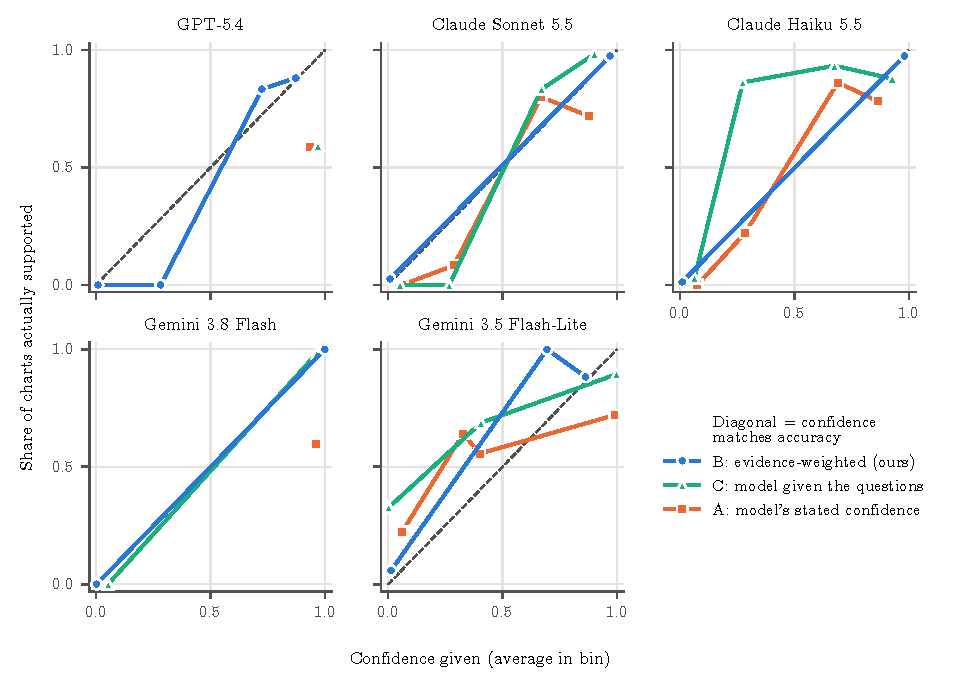
\includegraphics[width=\textwidth]{figures/reliability.pdf}
\caption{Reliability diagrams, study 3 test split: average confidence given in each of five bins (x) against the share of its charts actually supported (y); bins with fewer than 5 charts omitted. The dashed diagonal is perfect calibration. GPT-5.4 put almost every chart above 90\% under A and C, so each has a single point; on Gemini 3.8 Flash, B and C overlap.}\label{fig:reliability}
\end{figure}

\textbf{When B said 90\% or more, it was right 93--100\% of the time on every model}, within one percentage point of its stated confidence; when it said under 10\%, 0--6\% of charts were supported. The models' own confidence did not have this property: GPT-5.4 and Gemini 3.8 Flash put 149 and 183 of 200 charts above 90\%, and only 54\% and 63\% of those were supported. Recalibration repairs the average but a monotone map cannot improve ranking, so the recalibrated score crowds into the middle and almost never reaches 90\%. Giving the model the questions (C) produced honest high confidence on Sonnet and Gemini 3.8 Flash but not on the other three: GPT-5.4 said 97\% and was right 60\% of the time. The questions help the model reason; the fitted scoring is what makes the number trustworthy across models. At a 0.5 cut-off B also had the highest $F_{0.5}$ on four models (0.888--1.000) and was within 0.002 of C on Sonnet.

\subsection{Fix the questions, not the model}\label{sec:tuning}

Study 2 applied the frozen pilot pipeline to harder charts. B still ranked far better than stated confidence (AUROC 0.932 against 0.470 for GPT-5.4; 0.979 against 0.731 for Gemini 3.8 Flash), but it was blind to nurse-only visits, unsigned notes and chart-review e-consults: such notes satisfy every question of the six-question rubric, and the frozen B scored them 0.94 (GPT-5.4) and 0.99 (Gemini 3.8 Flash) on average. The evidence trail showed why: every high score had quotes for diabetes, CKD and a plan line, and none for a qualifying encounter or signature, because no question asked for one. Rubric version 3 added two gates for these rules (R1 and R2), with no change to any model. On the study-3 test split, \textbf{B scored all 26 such charts as unsupported on all five models}; C, given the same two questions, got 25 of 26 wrong on GPT-5.4 (Table~\ref{tab:families}).

\begin{table}[!htbp]
\centering\small
\caption{Charts wrong at a 0.5 cut-off, B / C, by family (study 3 test). F: outside the pilot rubric; G: borderline ``addressed'' wording; H: hard cases.}\label{tab:families}
\begin{tabular}{@{}lcccccccc@{}}
\toprule
Model & A (32) & B (27) & C (21) & D (15) & E (15) & F (26) & G (39) & H (25) \\
\midrule
GPT-5.4 & 3 / 14 & 0 / 0 & 0 / 12 & 2 / 9 & 0 / 0 & \textbf{0} / 25 & 9 / 9 & 5 / 11 \\
Claude Sonnet 5.5 & 2 / 0 & 0 / 0 & 0 / 0 & 0 / 0 & 0 / 0 & \textbf{0} / 0 & 1 / 2 & 2 / 2 \\
Claude Haiku 5.5 & 1 / 11 & 1 / 10 & 0 / 4 & 0 / 5 & 0 / 4 & \textbf{0} / 0 & 0 / 19 & 2 / 7 \\
Gemini 3.8 Flash & 0 / 0 & 0 / 0 & 0 / 0 & 0 / 1 & 0 / 0 & \textbf{0} / 0 & 0 / 1 & 0 / 0 \\
Gemini 3.5 Flash-Lite & 1 / 8 & 1 / 12 & 1 / 2 & 0 / 2 & 0 / 5 & \textbf{0} / 4 & 11 / 19 & 5 / 7 \\
\bottomrule
\end{tabular}
\end{table}

Most remaining errors are in family G on GPT-5.4 and Flash-Lite: reading ``see nephrology note'' as CKD addressed, or missing a medication change made for kidney function. Each shows up as a specific Q4 answer with its quote, so the fix is a targeted change to one question, tested on development data.

\subsection{Inexpensive models}\label{sec:cost}

Because the judgment sits in the questions and the fitted weights, a smaller model only has to read accurately. Claude Haiku 5.5 with EWC matched or exceeded Claude Sonnet 5.5 with EWC on every measure (AUROC 0.994 against 0.987, ECE 0.014 against 0.021; Tables~\ref{tab:main} and~\ref{tab:said}) at about one fifteenth of the cost: \$2.82 against \$43.82 for the full development and test run (3,850 calls each, at list prices), and was the only model to pass all four pre-registered checks. Gemini 3.5 Flash-Lite with EWC (AUROC 0.897) outranked every model's own stated confidence (best 0.772) and its 90\%+ scores were right 93\% of the time, but it was not accurate enough to auto-accept at 95\% precision; that shortfall was visible on development data before deployment.

\subsection{Extraction, ablations and fitted weights}

Extraction macro-$F_1$ against the intended answers was at least 0.97 on every question for Haiku and Gemini 3.8 Flash; the weakest questions were Q2 (eGFR dates; 0.743--0.857 on GPT-5.4, Sonnet and Flash-Lite) and R2 (signature; 0.848--0.895 on the same models). Quote verification failed for at most 0.5\% of answers, and the median standard deviation of B's score across five extraction runs was 0.000 on every model, so one extraction run is enough.

Table~\ref{tab:ablations} reports views computed from the same calls. Unfitted expert weights already rank well but are poorly calibrated, so fitting is what makes the score a probability. Collapsing \textit{no} and \nd{} lowered AUROC slightly on all five models. Removing quote verification changed little, because models almost never misquoted.

\begin{table}[!htbp]
\centering\small
\caption{Secondary views, study 3 test split: AUROC / ECE. Self-consistency is the share of the five stated-confidence runs calling the chart supported.}\label{tab:ablations}
\begin{tabular}{@{}lccccc@{}}
\toprule
View & GPT-5.4 & Sonnet 5.5 & Haiku 5.5 & Gemini 3.8 Flash & Flash-Lite \\
\midrule
B, fitted weights & 0.926 / 0.037 & 0.987 / 0.021 & 0.994 / 0.014 & 1.000 / 0.002 & 0.897 / 0.050 \\
Self-consistency & 0.588 / 0.445 & 0.873 / 0.104 & 0.879 / 0.111 & 0.890 / 0.095 & 0.650 / 0.326 \\
B, expert weights & 0.900 / 0.093 & 0.973 / 0.128 & 0.982 / 0.117 & 0.990 / 0.123 & 0.879 / 0.149 \\
B without quote verification & 0.926 / 0.037 & 0.987 / 0.021 & 0.994 / 0.010 & 1.000 / 0.002 & 0.919 / 0.041 \\
B with two-way answers & 0.921 / 0.033 & 0.983 / 0.027 & 0.989 / 0.014 & 0.988 / 0.002 & 0.894 / 0.029 \\
\bottomrule
\end{tabular}
\end{table}

The fitted weights put almost all the signal on Q4 (addressed this visit, $+2.4$ to $+12.5$) and on Q3 = no (another cause, $-1.6$ to $-10.4$). Q1 (stage documented) received a negative weight on every model; this does not mean a stage counts against the code, but that in these charts a stage often appears in unsupported notes (a staged CKD entry in a problem list that is not addressed), and once Q4 is in the model, ``stage documented'' mostly marks those notes. Jointly fitted weights share credit among correlated answers and should be read as a scoring device; the audit trail is the answers and quotes.

\subsection{What the results mean}

\textbf{For inexpensive models, the method makes them usable scorers}: Haiku with EWC matched the best frontier result, and Flash-Lite with EWC outranked every model's own confidence. \textbf{For frontier models, it matches their ranking and adds calibration and an audit trail}: given the same questions, Sonnet and Gemini 3.8 Flash ranked as well as EWC, and EWC added better calibration (ECE 0.021 against 0.090 and 0.002 against 0.036), a verified quote behind every answer and a reproducible score. It is also robust where prompting alone is not: the same criteria-guided prompt that matched EWC on Sonnet ranked worse than chance on GPT-5.4, so with EWC an organization does not need to know in advance which kind of model it has. Two levers produce these results: tuning the questions fixes what the rubric cannot see, and fitting the weights makes the score a probability.

\paragraph{Earlier studies.} In the pilot (rubric revised once on development data), B reached AUROC 0.969 and ECE 0.009 on GPT-5.4 and 0.979 and 0.016 on Gemini 3.8 Flash, against recalibrated stated confidence at 0.571 and 0.107, and 0.669 and 0.120. In the transfer test's first stage, B led stated confidence and criteria-guided confidence on GPT-5.4 (AUROC 0.932 against 0.470 and 0.441) and stated confidence on Gemini 3.8 Flash (0.979 against 0.731; C 0.961), and revealed the blind spot described in Section~\ref{sec:tuning}.

% ---------------------------------------------------------------------------
\section{Limitations and next steps}

\begin{itemize}
  \item \textbf{Synthetic charts.} Notes come from phrase banks and edited templates; real notes are longer, messier and more varied.
  \item \textbf{Labels favor the method by construction.} The labels follow mostly from the facts the rubric asks about; method C received the same questions to keep the comparison fair.
  \item \textbf{Same-family generation.} The charts were generated with Claude, and two Claude models were tested.
  \item \textbf{Prevalence.} 58\% of test charts are supported, far above a real population; the intercept can be shifted for deployment, but calibration must be rechecked on real data.
  \item \textbf{Small data, one code.} About 100 gate-passing development charts per model fitted the weights, and the strongest extractors nearly separated the classes; 200 test charts cannot resolve small differences.
  \item \textbf{No certified coder.} The label rules were set by the study lead with AI assistance and checked by a built-in checker (0 of 350 charts with problems; 6 of 6 planted errors caught) and a 74-chart review; no certified coder reviewed them. All methods are scored against the same labels, so this does not affect the comparison between them.
  \item \textbf{Deviations from the plan.} Self-consistency reused the stated-confidence runs; a tolerant JSON parse was declared before the first call for two models; one model's freeze and test collection were started together by mistake (all frozen files matched the development fit); study 2's second stage was not run; the confidence-versus-accuracy view and the reliability figure are exploratory.
  \item \textbf{Added models.} Three of the five models were added after the pre-registration, each under its own addendum filed before its first call.
  \item \textbf{Documented is not true, and quotes can be misread.} The score measures how well the note supports the code; verification catches invented quotes, not real quotes misread, which is where the remaining errors came from.
\end{itemize}

The rubric changes with the use case; the pipeline and the fitting do not. The same structure applies to prior authorization (policy criteria as gates), overpayment review and trial matching, and rubrics can be layered (generic, code-family and code-specific questions) so that rare codes borrow weights from their family. The next steps are real charts labeled by certified coders, more codes, a code-computed check of the clarity of each quote, and a second model that verifies whether each quote supports its answer.

% ---------------------------------------------------------------------------
\section{Conclusion}

A confidence number has meaning only when it is computed from checked evidence and tested against outcomes. Evidence-weighted confidence does both: the LLM supplies quoted answers to rule-derived questions, code verifies and encodes them, and a fitted logistic regression turns them into a probability. On synthetic E11.22 charts and five models, charts it scored 90\% or more were supported 93--100\% of the time, while the models' own 93--99\% was right 54--72\% of the time; it ranked better than the models' own confidence and was the best-calibrated method on every model; a blind spot was fixed by adding two questions; and an inexpensive model inside the method matched the best frontier result at a fraction of the cost.

% ---------------------------------------------------------------------------
\begin{thebibliography}{99}\small
\bibitem{xiong} Miao Xiong, Zhiyuan Hu, Xinyang Lu, Yifei Li, Jie Fu, Junxian He, and Bryan Hooi. Can LLMs express their uncertainty? An empirical evaluation of confidence elicitation in LLMs. In \emph{ICLR}, 2024. \url{https://arxiv.org/abs/2306.13063}.
\bibitem{leng} Jixuan Leng, Chengsong Huang, Banghua Zhu, and Jiaxin Huang. Taming overconfidence in LLMs: Reward calibration in RLHF. In \emph{ICLR}, 2025. \url{https://arxiv.org/abs/2410.09724}.
\bibitem{soroush} Ali Soroush et al. Large language models are poor medical coders: Benchmarking of medical code querying. \emph{NEJM AI}, 1(5), 2024. doi: 10.1056/AIdbp2300040.
\bibitem{platt} John C. Platt. Probabilistic outputs for support vector machines and comparisons to regularized likelihood methods. In \emph{Advances in Large Margin Classifiers}. MIT Press, 2000.
\bibitem{checkeval} Yukyung Lee, Joonghoon Kim, Jaehee Kim, Hyowon Cho, Jaewook Kang, Pilsung Kang, and Najoung Kim. CheckEval: A reliable LLM-as-a-judge framework for evaluating text generation using checklists. In \emph{EMNLP}, 2025. \url{https://arxiv.org/abs/2403.18771}.
\bibitem{cbm} Pang Wei Koh, Thao Nguyen, Yew Siang Tang, Stephen Mussmann, Emma Pierson, Been Kim, and Percy Liang. Concept bottleneck models. In \emph{ICML}, PMLR 119, 2020. \url{https://proceedings.mlr.press/v119/koh20a.html}.
\bibitem{good} I.~J. Good. \emph{Probability and the Weighing of Evidence}. Griffin, London, 1950.
\bibitem{zeinoun} Issam Zeinoun. Beyond accuracy: A risk-driven architecture for monitoring AI in prior authorization. Zenodo, 2026. \url{https://doi.org/10.5281/zenodo.23628695}.
\bibitem{ewc1} Issam Zeinoun. Evidence-weighted confidence: Auditable, calibrated scoring of LLM outputs (extended version, with the full method derivation and algorithm specification). Zenodo, 2026. doi: \href{https://doi.org/10.5281/zenodo.23651100}{10.5281/zenodo.23651100} (all versions).
\bibitem{guidelines} Centers for Medicare \& Medicaid Services and National Center for Health Statistics. ICD-10-CM official guidelines for coding and reporting, FY 2027, 2026. Effective October 1, 2026.
\bibitem{tabular} Centers for Medicare \& Medicaid Services. 2027 ICD-10-CM code tables, tabular and index, 2026. Tabular List entry for E11.22 and its instructional notes.
\end{thebibliography}

% ---------------------------------------------------------------------------
\appendix
\section{Rubric version 3: full guidance}\label{app:rubric}

Each question is answered yes, no or \nd{} with an exact quote. The guidance below (abridged) is given to the model with each question; method C received the same questions and guidance.

\begin{small}
\noindent\begin{tabularx}{\textwidth}{@{}p{0.6cm}L@{}}
\toprule
ID & Guidance \\
\midrule
G1 & Yes for type 2, or diabetes without a type (ICD-10-CM defaults to type 2); insulin use does not change the type. No for type 1, secondary diabetes (drug, chemical, another condition, a procedure such as pancreatectomy), or both type 1 and type 2 without saying which is correct. \\
G2 & Yes if CKD is diagnosed anywhere, including ESRD or stage 5, or a history of CKD managed at this visit. No if possible, suspected, rule out, ``CKD?'', deferred; if the current assessment questions or defers CKD although the problem list includes it; or if the note elsewhere says there is no kidney disease and does not resolve the contradiction. Not documented for abnormal labs only, ``kidneys OK'', or ``renal involvement'' without the words CKD or chronic kidney disease. \\
R1 & No if the visit was with a nurse, dietitian or other staff only, or the patient was not seen (chart review, e-consult). \\
R2 & Yes only if a signature line names the clinician with a credential such as MD, DO, NP, FNP-C or PA-C. No if unsigned, pending signature, or without a credential. \\
Q1 & Yes if a stage (3a, 3b, 4, 5 or ESRD) is stated anywhere, even if sections or labs disagree; otherwise not documented, not no. \\
Q2 & Yes if two results below 60 are dated at least 90 days apart; no only if the most recent eGFR is 60 or above; otherwise not documented. \\
Q3 & Yes if due to, secondary to or caused by diabetes, or diabetic kidney disease, including diabetes named with another cause or as the likely cause. No if attributed to a different cause instead of diabetes. Not documented if no cause is stated. \\
Q4 & Yes if CKD appears in the assessment and plan with any status, evaluation, plan or treatment, including a copied-forward line (``stable'', ``continue regimen'') or CKD in a list of chronic conditions reviewed in the plan; a medication change because of kidney function counts. Not documented if CKD appears only in the problem list or history, or the plan only refers to another clinician's note (``see nephrology note''). \\
\bottomrule
\end{tabularx}
\end{small}

\end{document}
